\subsection{半单代数的自同构}

定理 4. —— 设 A 是一个半单环，Z 是它的中心，u 是 A 的一个自同构。假设 A 是一个有限生成的 Z-模，且对 Z 中的每个 z 有 \(u(z) = z\)。则 u 是一个内自同构。

这由应用于 \(f = \mathrm{Id}_{\mathrm{A}}\) 与 \(g = u\) 的 VIII, 第 256 页的定理 2 得出。

例. —— 定理 4 适用于下面两个特殊情形：

\pandocbounded{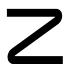
\includegraphics[keepaspectratio]{images/part002_1d1a6ca2.jpg}}

\begin{enumerate}
\def\labelenumi{\alph{enumi})}
\item
  设 D 是一个体，Z 是它的中心。若 D 在 Z 上是有限次数的，则 D 的每个固定 Z 中元素的自同构都是内自同构。D 在 Z 上是有限次数的这一假设是本质的（VIII, 第 269 页，习题 4）。
\item
  设 V 是域 K 上的一个有限维向量空间。K-代数 \(\operatorname{End}_{\mathrm{K}}(\mathrm{V})\) 的每个自同构都是内自同构；这一结果可以推广到向量空间 V 在 K 上不是有限维的情形（VIII, 第 272 页，习题 13）。
\end{enumerate}

特别地，矩阵代数 \(\mathbf{M}_{n}(\mathrm{K})\)（其中 \(n \geqslant 1\)）的每个自同构都是内自同构。这一结果有如下的推广。

命题 2. —— 设 L 是一个交换环，V 是一个维数为 m 的自由 L-模。假设每个使得 \(M^{m}\) 同构于 \(L^{m}\) 的 L-模 M 都同构于 L。则 L-代数 \(\operatorname{End}_{\mathrm{L}}(\mathrm{V})\) 的每个自同构都是内自同构。

设 \(B = \text{End}_{\text{L}}(\text{V})\)。设 u 是 L-代数 B 的一个自同构。我们把 V 视为一个左 B-模；用 \(u_{*}(\text{V})\) 表示与 u 相伴的左 B-模，其外部律为 \((b, v) \mapsto u(b)(v)\)（II, §1, No.~13, 第 221 页）。设 \((e_1, \ldots, e_m)\) 是 L-模 V 的一个基；给定 V 的元素 \(v_1, \ldots, v_m\)，存在 B 的唯一元素 b，使得我们有 \(b(e_i) = v_i\)（对 \(1 \leqslant i \leqslant m\)）。换句话说，元素 \(e = (e_1, \ldots, e_m)\)（\(V^m\) 的）给出 B-模 \(V^m\) 的一个基。由于 u 是自同构，e 也给出 B-模 \(u_{*}(\text{V}^m) = u_{*}(\text{V})^m\) 的一个基，因而该模同构于 \(V^m\)。(B, L)-双模 V 是可逆的（VIII, 第 102 页，例 1）。于是，由 VIII, 第 103 页的定理 2, b)，存在一个 L-模 M，使得 B-模 \(u_{*}(\text{V})\) 同构于 \(V \otimes_{L} M\)。因此，B-模 \(V \otimes_{L} L^m\) 与 \(V \otimes_{L} M^m\)（分别同构于 \(V^m\) 与 \(u_{*}(\text{V})^m\)）是同构的。由同上，L-模 \(L^m\) 与 \(M^m\) 同构。根据假设，M 同构于 L；于是，B-模 \(u_{*}(\text{V})\)（它同构于 \(V \otimes_{L} M\)）同构于 V。设 h 是从 V 到 \(u_{*}(\text{V})\) 的一个 B-模同构；它特别是 L-模 V 的一个自同构，即 B 的一个可逆元素。对 B 中的 b 与 V 中的 v，我们有 \(h(b(v)) = u(b)(h(v))\)，因此 \(u(b) = hbh^{-1}\)。

特别地，当交换环 L 是主理想整环（VII, §3, 第 15 页，推论 3）、是阿廷环（VIII, 第 37 页，定理 2, d)）或是局部环（VIII, 第 36 页，推论 6）时，命题 2 的条件得到满足。

